% !TEX root = ../main.tex
\section{Approach}
\label{sec:approach}
This section describes a method for estimating poses of noisy square fiducial tags using RGBD data. Unlike previous methods, the detected corners of the tag are treated as approximated locations of the true corners. Using the corners, the method implicitly evaluate the depth data and RGB data as two independent observations and fuse them in a meaningful way.

There are three distinct components to this method. First, we find the plane in $SO(3)$ containing the tag using depth data. Second, an approximate pose is computed using the depth plane and the corners from tag detection. Finally, the method refines the initial pose using the RGB data. Each component is described in detail in the following subsections and illustrated in Fig. 

\subsection{Depth Plane Fitting}
Since the fiducial tags are planar, we can obtain the pose the tag using a depth sensor by fitting a plane over the depth points. Although the corners of the fiducial tags found in the RGB images might be noisy, they are accurate enough to locate the region of the tag offset by at most a few pixels. With a calibrated RGBD sensor, we can extract the patch of depth points containing the planar tag. 

The raw range data retrieved from the Kinect One sensor are usually far from perfect for fitting an exact plane. Specifically, borders of the tag and some of the dark regions of the tag produce highly unreliable range data. Therefore, we first filter the data by removing points too far from the median before fitting the plane. Furthermore, the remaining points could have a large variance depending on the background lighting and the magnitude of the plane rotation. In the cases where depth sensor are noisy, we want to lower the weight of our initial pose estimate later in the pipeline. 

In implementation, we used a Bayesian plane fitting algorithm (describe the algorithm below) which assumes some noise model of the data and computes the mean and covariance of the plane. The noise model we used is a Kinect specific noise model [reference], which increases with the axis rotation of the depth plane. Note that a higher covariance implies that we are more uncertain about our fitting plane.

\begin{figure}
\centering
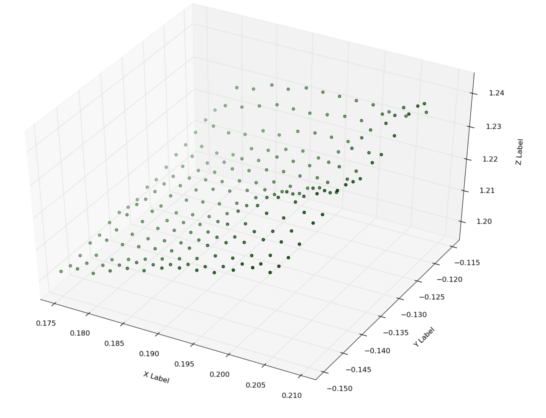
\includegraphics[width=\columnwidth]{figs/depth_plane_fig}
\caption{The depth points of the Apriltag plane. The points are noisy but good for an approximate estimation.}
\label{fig:calib}
\end{figure}

\subsection{Initial Pose Estimation}
The pose of the tag can be described as the transformation from tag's frame to the sensory frame of the robot given by $[R, \boldsymbol{t}]$. However, the depth plane $D [ \boldsymbol{\hat{n}}, d]$ and alone is insufficient to determine the transformation because it defines only 3 DOF. Furthermore, the center of the tag must align with the center of the plane and it further constrain 2 DOF. However, there are still infinite number of valid poses rotating about the normal $\boldsymbol{\hat{n}}$. One solution is to further constrain the pose by using a corner as an extra point correspondence to solve for the optimal rotation. However, the accuracy of this method largely depends on the depth accuracy of the chosen corner point. 

An alternative is to use all four detected corners as point correspondences for the optimization. We projected the detected corners onto $D [ \boldsymbol{\hat{n}}, d]$ to the coordinates, $p_i$, in the robot sensory frame. From here, the pose of the tag can be described as the homogenious transformation from the tag frame to the camera frame. We can solve for the transformation with a set of two 3D point correspondences: the projected points of the tag in the camera frame and the points in the tag frame. The points in the camera frame would be the projected corners which form a $4x3$ matrix of homogeneous points denoted as $p_i$. The points, $q_i$ in the tag frame are the coordinate of the four corners measured from the center of the tag with depth of 0 because they are planar. We can formulate this to be a 3D rigid body transformation estimation problem [Reference to SVD 3D rigid body]. Solving for the optimal transformation $[R, \boldsymbol{t}]$ requires minimizing a least squares error objective function given by:
\begin{IEEEeqnarray}{c}
[R, \boldsymbol{t}] = \argmin _{R \in SO(3), \boldsymbol{t}\in \mathbb{R}^3} \sum_{i=1}^{n} w_i \| R \boldsymbol{p_i} + \boldsymbol{t} - \boldsymbol{q_i}\| ^2
\IEEEeqnarraynumspace
\label{eq:rigid_body}
\end{IEEEeqnarray}
There are numerous approaches to solve Eq. \ref{eq:rigid_body}. Since we have very few correspondences and they are assumed to be correct, it can be computed quickly using SVD:
\begin{IEEEeqnarray}{rCl}
& \bar{p} = \frac{1}{N} \sum_{i=1}^{N} p_i \qquad p_{ci} = p_i - \bar{p} \\
& \bar{q} = \frac{1}{N} \sum_{i=1}^{N} q_i \qquad q_{ci} = q_i - \bar{q} 
\end{IEEEeqnarray}
\begin{IEEEeqnarray}{rCl}
p_{c}^{\top}q_c &= U\Sigma V^\top \\
R & = VU^\top\\
\boldsymbol{t} & = \bar{q} - R\bar{p}
\end{IEEEeqnarray}
$R$ and $t$ are the rotation and translation components of the the homogenous transform. When we project the points onto the depth plane, the squares will likely deform. Therefore, we use the above algorithm to find the optimal transformation $H$ that minimizes the error in the least square sense. 
The pose obtained from the range data, although not always accurate, is consistent under noise and does not suffer from the perceptual ambiguity problem. 
\subsection{Pose Refinement}
\begin{figure}
\centering
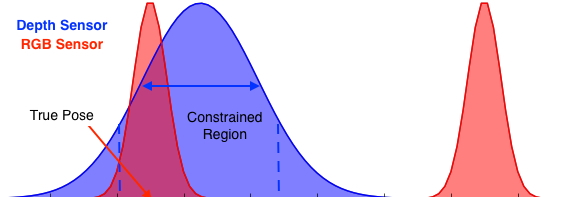
\includegraphics[width=\columnwidth]{figs/optimization_visualization_fig}
\caption{An abstract visualization of the optimization constraints. The blue curve is the initial pose estimation obtained from the depth plane. The red curves are the ambiguous poses from the RGB image. We constrained the region of optimization based on how well we fit the depth plane.}
\label{fig:calib}
\end{figure}
Given the initial pose estimate of the tag and the RGB image, we can refine the pose that minimizes the reprojection error. Given camera model $K$, initial rotation and translation estimates $R_{init}$ and $t_{init}$
\begin{align*}
\hat{y} &= K[(R_{init} + \Delta R)x + (t_{init} + \Delta t)]\\
&\underset{\Delta R, \Delta t}{\mathrm{min}} (y - \hat{y})\\
&\text{subject to:} \\
& |\Delta R| <= \Gamma_R, \; |\Delta t| <= \Gamma_t\\
\end{align*}
The challenge here is to determine the region $\Gamma_R$ and $\Gamma_t$ which the initial pose estimate can be adjusted. If we unbound $\Delta R$ and $\Delta t$ intheon Apriltag detection algorithmson Apriltag detection algorithm the optimization, the solution might converge to a pose optimal for the reprojection error but far away from the true pose due to perceptual ambiguity. On the other hand, if we constrain the optimization too much, the final pose might not be far away from the true pose because of the inaccurate initial estimation. We recognize that the bound of on this optimization is related to the variance of the initial pose estimation. In one extreme, if there is no uncertainty in the depth camera and the range data are perfect, we don't need to further refine the pose of the tag. Similarly, if we don't have any depth information (uncertainty of the initial estimate is infinity), then the best we can do is find the pose solely based on the reprojection error which is the same as solving the unbounded optimization problem. Thererfore, this becomes a constrained optimization problem where the bound on the independent variables of $\Delta R$ and $\Delta t$ is proportional to the covariance of our estimated depth plane parameters. In our implementation, we used the trust-region algorithm to bound the optimization. The scaling threshold parameter is emperically tested to yield the best results for our robot. 

The key insight to our method is that it harness the different strength of RGB and depth information during the pose optimization process. By considering all the points on the tag, the depth data is more robust to noises in the scene. However, range data is inherently inconsistent and the pose is thus imprecise. In contrast, the advantage of RGB image is that the corners can be detected at a sub-pixel precision. It is useful for refinement optimization.  